\begin{center}
    \textbf{\huge Лабораторная работа №1}
    
    \textbf{\large Численное дифференцирование}
\end{center}

\section{Введение}
Рассмотрим произвольную достаточно гладкую функцию $f(x)$, определённую на отрезке $\sqbrk{a, b}$ вместе с первой и второй производной.
Сопоставим ей сеточную функцию $f[x_i]$, определённую на множестве точек $a = x_0 < x_1 < \ldots < x_{N-1} < x_N - b$.
Воспользуемся формулами численного дифференцирования разного порядка аппроксимации для вычисления первой и второй производных сеточной функции:

Формулы первого порядка:
\begin{gather*}
    f'[x_i] \approx \frac{f[x_{i+1}] - f[x_i]}{h} \textrm{ --- производная вперёд;} \\
    f'[x_i] \approx \frac{f[x_i] - f[x_{i-1}]}{h} \textrm{ --- производная назад.}
\end{gather*}
Если $\exists M_2 : \forall \xi \in \sqbrk{a, b} \rightarrow \left| f''(\xi) \right| \leqslant M_2$, то погрешность этой формулы имеет первый порядок по $h$:
\[
    \left| r_1 \right| = \left| f'(\xi) - \frac{f(\xi + h) - f(\xi)}{h} \right| \leqslant \frac{M_2 h}{2}.
\]

Формула второго порядка аппроксимации:
\[
    f'[x_i] \approx \frac{f[x_{i+1}] - f[x_{i-1}]}{2h}.
\]
Если $\exists M_3 : \forall \xi \in \sqbrk{a, b} \rightarrow \left| f'''(\xi) \right| \leqslant M_2$, то погрешность этой формулы имеет второй порядок по $h$:
\[
    \left| r_1 \right| =  \left| f'(\xi) - \frac{f(\xi + h) - f(\xi - h)}{2h}  \right| \leqslant \frac{M_3 h^2}{6}.
\]
На концах отрезка формула второго порядка имеет вид:
\begin{gather*}
    f'[x_0] \approx \frac{-3f[x_0] + 4f[x_1] - f[x_2]}{2h}, \\
    f'[x_N] \approx \frac{3f[x_N] - 4f[x_{N-1}] + f[x_{N-2}]}{2h}, \\
\end{gather*}

Формула для вычисления второй производной:
\[
    f''(x_i) \approx \frac{f[x_{i+1}] - 2f[x_i] + f[x_{i-1}]}{h^2}
\]
На концах отрезка формула принимает вид
\begin{gather*}
    f''[x_0] \approx \frac{2f[x_0] - 5f[x_1] + 4f[x_2] -f[x_3]}{h^2}, \\
    f''[x_N] \approx \frac{2f[x_N] - 5f[x_{N-1}] + 4f[x_{N-2}] -f[x_{N-3}]}{h^2}
\end{gather*}

\section{Выполнение работы}
Проверим порядок стремления к нулю погрешности вычисления производных по данным формулам. Для этого
\begin{enumerate}
    \item Выберем некоторую гладкую функцию $f(x)$, найдём аналитически её первую и вторую производные.
    \item Зафиксируем отрезок $\sqbrk{a, b}$ и, варьируя $N$ --- число отрезков разбиения (в этом случае $h = \frac{1}{N}$), выполним следующие вычисления:
    \begin{enumerate}
        \item Спроектируем $f(x)$ на получившуюсся сетку $a = x_0 < x_1 < \ldots < x_{N-1} < x_N - b$.
        \item В каждой точке сетки численно найдём производные по всем трём методам.
        \item Найдём погрешность численного дифференцирования как наибольшее отклонение численной производной от проекции найденной аналитически производной на сетку.
    \end{enumerate}
    Построим зависимость логарифма погрешности от логарифма $N$, и по угловым коэффициентам прямых найдём фактический порядок аппроксимации.
\end{enumerate}
Вычисленные по линейному приближению порядки составили для фуyкции $\cos(x), x \in \sqbrk{-4, 4}$:
\begin{itemize}
    \item $n_{11} = 0.997$ --- для первой производной, метод первого порядка;
    \item $n_{12} = 1.941$ --- для первой производной, метод второго порядка;
    \item $n_{22} = 2.058$ -- вторая производная.
\end{itemize}

\begin{figure}[h]
    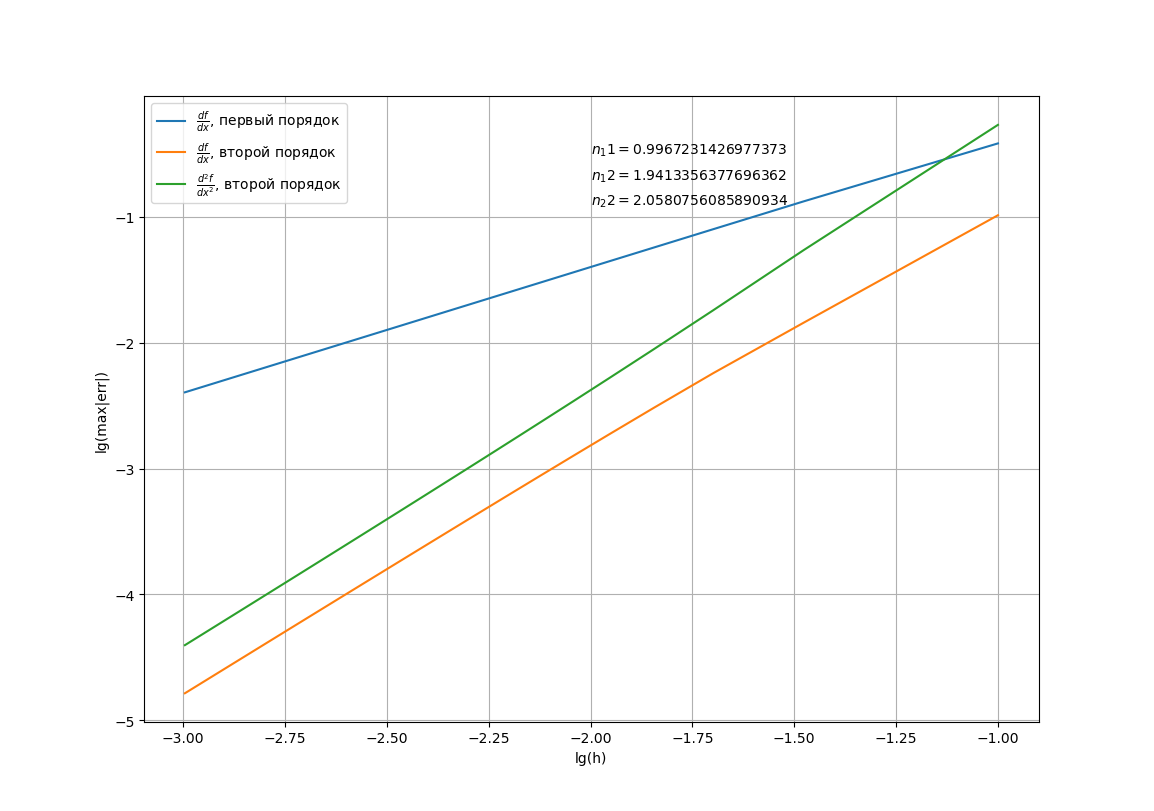
\includegraphics[width=\textwidth]{Figure_1.png}
    \caption{Зависимость погрешности от шага сетки}
\end{figure}